\title{PEC: Videojuegos 3D}
\author{David Morcillo}
\date{}

\documentclass[12pt]{article}
\usepackage[utf8]{inputenc}
\usepackage[pdftex]{graphicx}
\usepackage{parskip}
\usepackage{url}
\usepackage{setspace}

\begin{document}
\maketitle

\tableofcontents

\section{Introducción}

En este módulo teníamos que escoger entre cuatro opciones muy diferentes entre ellas. Después de pensarlo a conciencia decidí decantarme por la opción de trabajar con un motor físico existente.

Cuando pienso en un motor físico el primero que me viene a la cabeza es \textit{PhysX} de NVIDIA, quizás por ser el motor más usado en los videojuegos que he estado jugando últimamente. Decidí empezar por la documentación de \textit{PhysX}, pues ya conocía varios proyectos y sabía de lo que era capaz. Mi primera sorpresa fue que necesitaba una cuenta de desarrollador. Enviando un sencillo formulario conseguí acceder a la sección para desarrolladores y conseguí descargar el SDK.

Suelo trabajar en un sistema Linux y tuve algunos problemas con la nueva versión del SDK, así que busqué una versión más antigua y conseguí compilar algunas \textit{demos}. A mi pesar, la documentación de esa versión estaba obsoleta y la nueva documentación del SDK no me permitía bien seguir el código. Tras una lectura diagonal de la documentación decidí dejar \textit{PhysX} a un lado, pues no me acabó de convencer su soporte para mi plataforma de trabajo.

Buscando una alternativa encontré a \textit{Bullet}, una motor físico \textit{open source} y decidí empezar a trabajar con él.

\section{Motor físico: Bullet}

\textit{Bullet} es un motor para trabajar con colisiones, objetos rígidos y objectos ``blandos''. Se describe así mismo como una librería formada por varios módulos donde el programador podrá escoger usar alguno de ellos o bien usarlos todos en conjunto.

\subsection{Características}

Las características principales del motor son las siguientes:
\begin{itemize}
  \item \textbf{\textit{Open source}}: \textit{Bullet} se distribuye bajo la licencia Zlib y es gratuito para su uso comercial en muchas plataformas, incluyendo PLAYSTATION 3, XBox360, Wii, PC y iPhone. Algunos de los videojuegos en los que se ha usado son:
    \begin{itemize}
      \item Toy Story 3: The Video Game published by Disney Interactive Studios.
      \item Grand Theft Auto IV and Red Dead Redemption by Rockstar Games.
      \item Trials HD by RedLynx.
    \end{itemize}
  \item \textbf{Detección de colisiones}: tanto a nivel continuo como a nivel discreto. Incluye algoritmos como \textit{ray sweep test} y \textit{convex sweep test}. Podremos usar primitivas básicas como esferas, cubos y capsulas; también dispondremos de formas más complejas como mallas cóncavas y convexas.
  \item \textbf{Objetos rígidos}: Resolución rápida y estable de restricciones entre objetos rígidos, dinámica de vehículos, controladores de personaje. Algunas de las restricciones que podremos usar son: punto a punto, \textit{slider}, \textit{hinge}, genéricas 6DOF y \textit{cone twist} para el uso de \textit{ragdolls}.
  \item \textbf{Objetos blandos}: Simulación de telas, cuerdas y volúmenes deformables. 
  \item \textbf{Integraciones}: Maya, Blender y COLLADA.
\end{itemize}

\subsection{Diseño}

Tal y como hemos comentado con anterioridad, el motor esta diseñado para poder usar algunos de sus componentes sin necesidad de usar toda la librería. Podemos ver la organización de sus módulos en la figura \ref{fig:diseno}.

\begin{figure}[h]
\begin{center}
 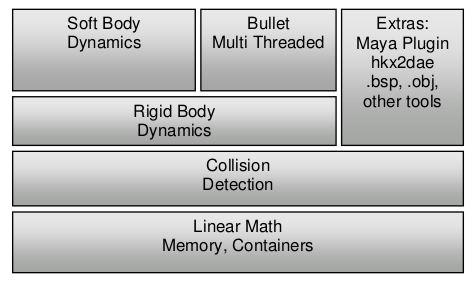
\includegraphics[width=10cm]{figures/diseno.png}
 \caption{Arquitectura de \textit{Bullet}}
 \label{fig:diseno}
\end{center}
\end{figure}

En esta práctica me he centrado principalmente en los módulos de \texttt{Rigid Body Dynamics} y \texttt{Collision Detection}. Para entender correctamente como interactúan estos dos módulos debemos analizar ahora el \texttt{Rigid Body Physics Pipeline}:

\begin{enumerate}
  \item Se aplica la fuerza de la gravedad a todos los objetos dinámicos de la escena.
  \item Se utiliza un primer algoritmo de detección de colisiones a \textit{grosso modo} en la \textit{Broadphase}. Los algoritmos usados por \textit{Bullet} son \textit{Dynamic AABB Tree} y \textit{Sweep and Prune (SAP)}. La salida del algoritmo es una colección de parejas de colisiones que se analizaran en la siguiente fase para detectar si hay colisión o no entre esos objetos.
  \item Se utiliza un algoritmo de granularidad más fina en la \textit{NarrowPhase}. En esta fase sabremos si dos objetos han tenido contacto o no.
  \item Finalmente se aplican las restricciones y se realiza una interpolación de la posición.
\end{enumerate}

\section{Proyectos}

En esta sección analizaremos algunos aspectos de la librería mediante algunos ejemplos de código usados en los proyectos realizados.

\subsection{\texttt{HelloWorld}}

Cuando empezamos a usar un nuevo lenguaje de programación o una librería, el primer programa que realizamos es el ``Hola Mundo!''. El programa que me proponía \textit{Bullet} era lanzar una pelota desde 50 metros y ver como actuaba la fuerza de la gravedad sobre ella hasta y finalmente colisionar contra el suelo.

El programa original solo mostraba la posición de la esfera en cada \textit{tick} pero para adaptarme a la práctica decidí usar OpenGL para la visualización de la simulación. En la figura \ref{fig:helloworld} podemos ver el resultado.

\begin{figure}[h]
\begin{center}
 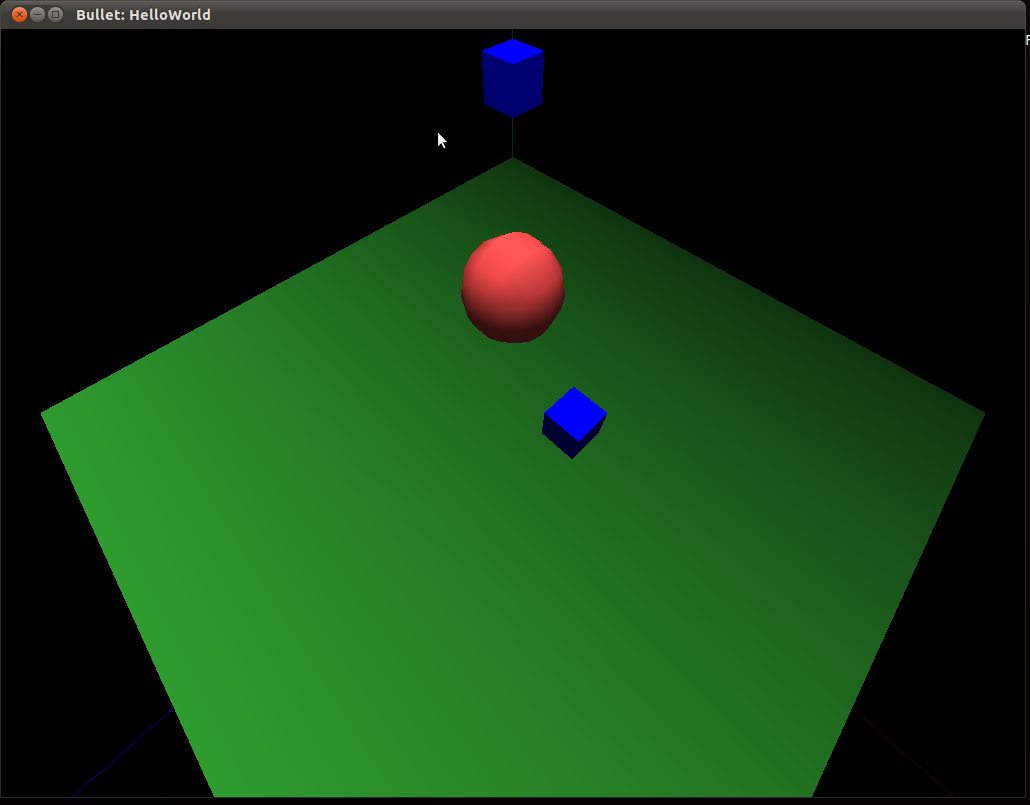
\includegraphics[width=10cm]{figures/helloworld.png}
 \caption{Proyecto \texttt{HelloWorld}}
 \label{fig:helloworld}
\end{center}
\end{figure}

Empecé a escribir todo el código realizado con la librería en una clase aparte llamada \texttt{PhysicsManager}. En primer lugar tenía que crear el mundo donde realizaría la simulación y asignarle un vector para la gravedad:

{\scriptsize
\begin{verbatim}
dynamicsWorld = new btDiscreteDynamicsWorld(dispatcher,broadphase,solver,collisionConfiguration);
dynamicsWorld->setGravity(btVector3(0,-10,0));
\end{verbatim}
}

En el ejemplo vemos como hemos creado un objeto de la clase \texttt{btDiscreteDynamicsWorld}. Al constructor del objeto le hemos pasado todos los elementos necesarios para la detección de colisiones:
\begin{itemize}
  \item \texttt{broadphase}: El objeto responsable de la detección de colisiones en la \textit{Broadphase}.
  \item \texttt{dispatcher} y \texttt{collisionConfiguration}: Responsables de la detección de contactos en la \textit{NarrowPhase}.
  \item \texttt{solver}: Se encarga de resolver las restricciones.
\end{itemize}

Una vez tenemos creado el mundo donde van a colisionar nuestros objetos tenemos que crear los objetos en sí. Para este proyecto se han usado dos objetos:
\begin{itemize}
  \item Una esfera de 1kg situada a 50 metros sobre el suelo.
  \item Un plano para representar el suelo.
\end{itemize}

No entraremos en detalle en la creación de dichos objetos ya que lo comentaremos en las siguientes secciones.

Finalmente, para realizar la simulación es necesario llamar al método \texttt{stepSimulation} de nuestro mundo en cada \textit{tick}:

{\scriptsize
\begin{verbatim}
void PhysicsManager::simulate(float dt)
{
  dynamicsWorld->stepSimulation(dt,10);
}
\end{verbatim}
}

\subsection{\texttt{Scene}}

En este proyecto debía representar una escena con varios objetos interactuando entre sí. El resultado lo podemos ver en la figura \ref{fig:scene}.

\begin{figure}[h]
\begin{center}
 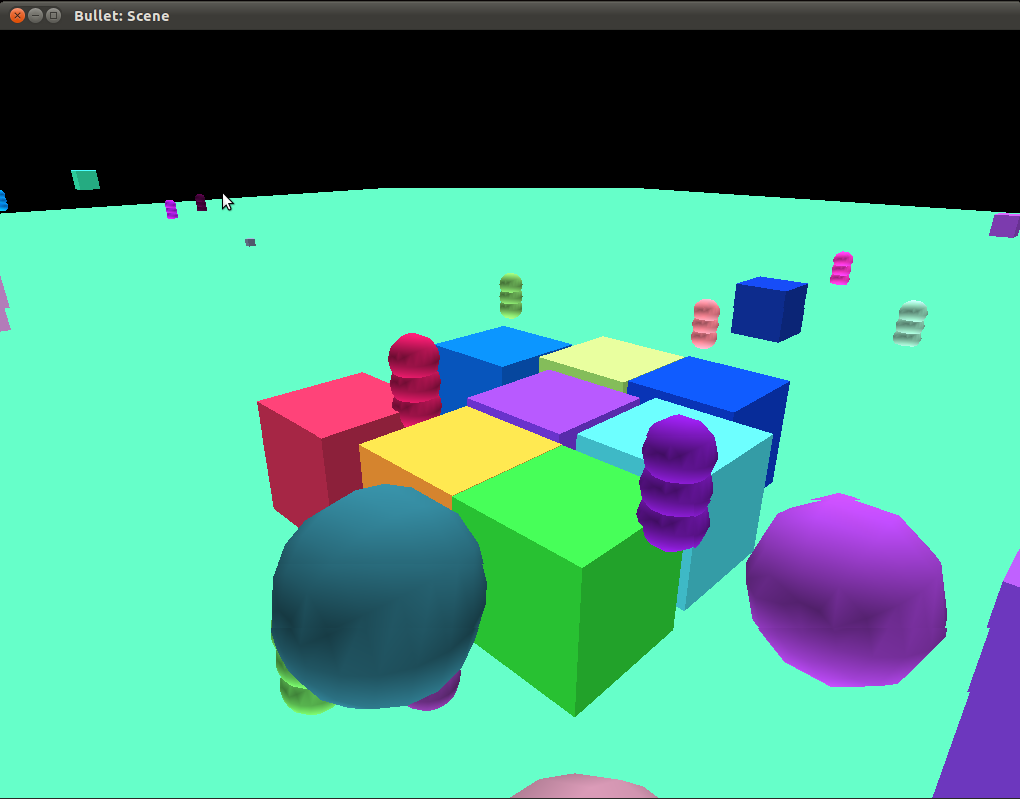
\includegraphics[width=10cm]{figures/scene.png}
 \caption{Proyecto \texttt{Scene}}
 \label{fig:scene}
\end{center}
\end{figure}

A nivel de código en este proyecto empecé a organizar un poco los objetos del mundo y cree la clase \texttt{Entity} y algunas subclases para representar los diferentes objetos: \texttt{Sphere}, \texttt{Box}, \texttt{Capsule} y \texttt{Ground}.

Cada entidad está formada por una forma y un cuerpo rígido. Usando la clase \texttt{PhysicsManager} escribí el código necesario para utilizar \texttt{Bullet}. Veamos el código para crear un cuerpo rígido:

{\scriptsize
\begin{verbatim}
btRigidBody* PhysicsManager::createRigidBody(btCollisionShape* shape, btVector3 position, btScalar mass)
{
  btDefaultMotionState* motionState;
  btRigidBody* rigidBody;

  motionState = new btDefaultMotionState(btTransform(btQuaternion(0,0,0,1), position));

  btVector3 inertia(0,0,0);
  shape->calculateLocalInertia(mass,inertia);

  btRigidBody::btRigidBodyConstructionInfo rigidBodyCI(mass,motionState,shape,inertia);
  rigidBody = new btRigidBody(rigidBodyCI);

  dynamicsWorld->addRigidBody(rigidBody);
  return rigidBody;
}
\end{verbatim}
}

Esta función recibe tres parámetros:
\begin{itemize}
  \item \texttt{btCollisionShape* shape}: Es el objeto base para representar una forma en \textit{Bullet}. El motor dispone de algunas primitivas básicas que hemos usado para nuestro proyecto, como por ejemplo \texttt{btSphereShape} y \texttt{btBoxShape}. Algunos objetos pueden compartir la forma pero el cuerpo rígido deberá ser diferente para cada uno.
  \item \texttt{btVector3 position}: La posición inicial de nuestro objeto. En la función se introduce el elemento \texttt{btDefaultMotionState}. Este objeto nos ahorrará mucho trabajo ya que \textit{Bullet} realizara todas las transformaciones de la posición del objeto sobre él, incluida la interpolación de posiciones entre paso y paso de la simulación.
  \item \texttt{btScalar mass}: La masa del objeto. Los objetos estáticos siempre tendrán masa 0 mientras que los objetos dinámicos deberán tener masa $>0$. En nuestro proyecto, el plano estático tiene masa 0kg mientras que los demás objetos tiene masa 1kg.
\end{itemize}

Nuestra clase \texttt{Entity} dispone de un apuntador para la forma y un apuntador para el cuerpo rígido. De esta forma podemos reutilizar la forma del objeto si es necesario.

\subsection{\texttt{AngryBlocks}}

Este proyecto es un prototipo de un mini-juego donde la física tiene un papel importante. En un principio, tal y como su nombre indica, debía tener ciertas similitudes con el conocido Angry Birds de Rovio. Aún así, por falta de tiempo y experiencia con el motor no ha sido posible el primer planteamiento del juego.

El nuevo diseño del juego es algo distinto y tiene ciertas similitudes con el juego de mesa Jenga. Podemos ver el resultado en la figura \ref{fig:angryblocks}.

\begin{figure}[h]
\begin{center}
 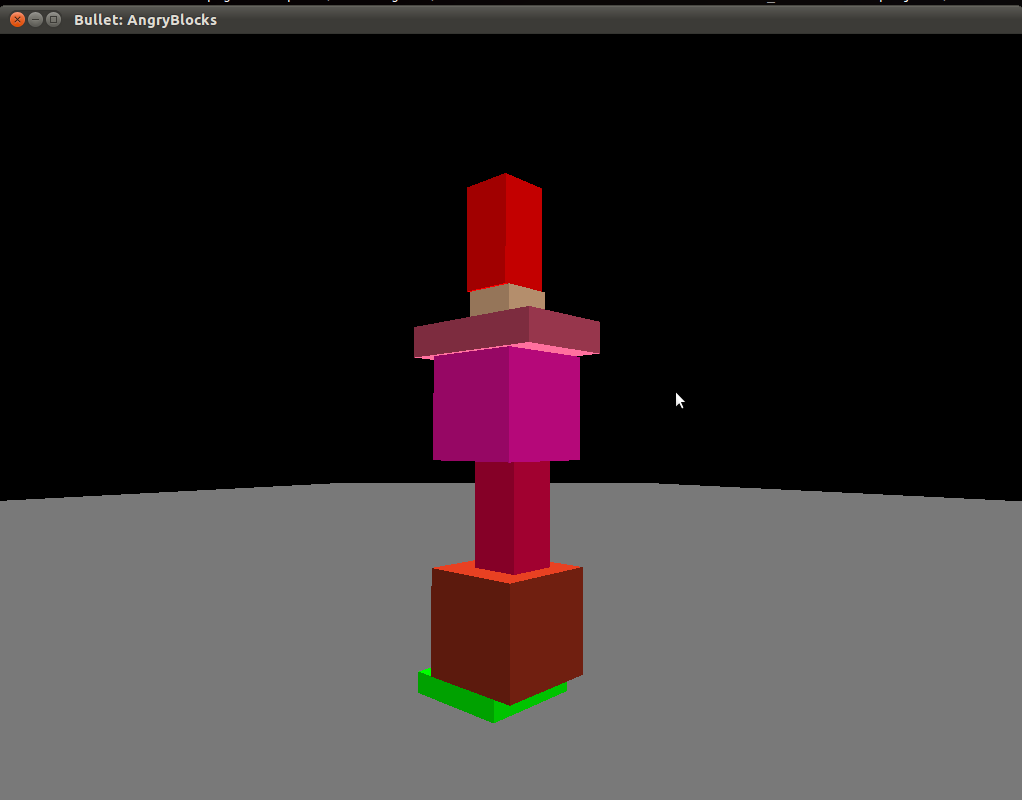
\includegraphics[width=10cm]{figures/angryblocks.png}
 \caption{Proyecto \texttt{AngryBlocks}}
 \label{fig:angryblocks}
\end{center}
\end{figure}

El objetivo del juego consiste en ir quitando las piezas de forma que la pieza roja consiga colisionar con la pieza verde. En este prototipo solo se ha realizado una fase a modo de ejemplo.

En el juego, el jugador solo puede mover la pieza que este en contacto directo con la pieza roja usando las teclas J, K, L y M (se han usado estas teclas para hacer un símil con el editor de texto VIM).

Se ha usado el código generado en los anteriores proyectos añadiendo una clase extra para gestionar las colisiones. \textit{Bullet} nos proporciona muchos mecanismos para filtrar y detectar colisiones. En este proyecto yo he usado una clase que deriva de \texttt{btOverlapFilterCallback}. Implementado el método \texttt{needBroadphaseCollision} podemos filtrar algunas colisiones en la \textit{Broadphase}. Veamos un fragmento del código:

{\scriptsize
\begin{verbatim}
bool CollisionFilter::needBroadphaseCollision(btBroadphaseProxy* proxy0,btBroadphaseProxy* proxy1) const
{
  if(game_logic->getTarget() != 0 && game_logic->getObjective() != 0)
  {
    btRigidBody* body0 = (btRigidBody*) proxy0->m_clientObject;
    btRigidBody* body1 = (btRigidBody*) proxy1->m_clientObject;
    (...)
  }
  return true;
}
\end{verbatim}
}

Se ha omitido parte del código que corresponde a la lógica de juego. En la función podemos ver como \textit{Bullet} nos proporciona dos objetos \texttt{proxy} que corresponden a dos objetos que van a colisionar en la \textit{Broadphase}.

\section{Conclusiones}

En esta práctica he hecho mis primeros pasos usando un motor físico. Es un \textit{software} complejo donde se necesitan buenos conocimientos de trigonometría y álgebra para poder llegar a entender todos los conceptos.

No he podido profundizar mucho en la librería pues el código es muy complejo y la documentación no es del todo exhaustiva. Aún así, la librería tiene un buen soporte y dispone de un foro con usuarios muy activos para resolver dudas y compartir opiniones.
Me hubiera gustado trabajar en algunos aspectos más avanzados, como por ejemplo la simulación de objetos ``blandos''. Es un tema que me llama mucho la atención y creo que añade mucho realismo al videojuego.

Para finalizar las conclusiones hablaremos sobre los pros y contras del motor utilizado y también analizaremos algunas ampliaciones y mejoras que se podrían realizar al mini-juego planteado.

\subsection{Ventajas e inconvenientes}

\subsubsection{Ventajas}

\begin{itemize}
  \item Modular: podemos usar algunas características del motor junto con nuestro programa.
  \item Fácil para empezar. Permite realizar un primer ejemplo en pocos pasos.
  \item Multiplataforma
\end{itemize}

\subsubsection{Inconvenientes}

\begin{itemize}
  \item La documentación es muy general y se necesitan muchos conocimientos previos.
  \item Poca variedad de restricciones.
\end{itemize}

\subsection{Ampliaciones}

\begin{itemize}
  \item Añadir más niveles con mayor dificultad.
  \item Añadir sombras.
  \item Varios objetivos.
  \item Multijugador: mover las piezas por turnos.
\end{itemize}

\end{document}
